% ============================================================
%  Smart Classroom Occupancy System – LaTeX Report
%  Author: Anshul (22DCS003)
%  NIT Hamirpur, CS-744 IoT, 2026
% ============================================================
\documentclass[12pt,a4paper]{article}

% ── Encoding & Language ─────────────────────────────────────
\usepackage[utf8]{inputenc}
\usepackage[T1]{fontenc}
\usepackage[english]{babel}

% ── Typography ───────────────────────────────────────────────
\usepackage{lmodern}
\usepackage{microtype}

% ── Page Layout ─────────────────────────────────────────────
\usepackage[
  top=25mm, bottom=25mm,
  left=25mm, right=25mm,
  headheight=14pt
]{geometry}

% ── Header / Footer ──────────────────────────────────────────
\usepackage{fancyhdr}
\pagestyle{fancy}
\fancyhf{}
\renewcommand{\headrulewidth}{0.4pt}
\fancyhead[L]{\small Smart Classroom Occupancy System}
\fancyhead[R]{\small NIT Hamirpur, 2026}
\fancyfoot[C]{\thepage}

% ── Mathematics ──────────────────────────────────────────────
\usepackage{amsmath,amssymb}

% ── Graphics & Colours ───────────────────────────────────────
\usepackage{graphicx}
\usepackage[dvipsnames,svgnames,x11names]{xcolor}

% ── TikZ for diagrams ────────────────────────────────────────
\usepackage{tikz}
\usetikzlibrary{
  shapes.geometric, shapes.misc,
  arrows.meta, arrows,
  positioning, fit,
  calc, decorations.pathmorphing,
  backgrounds, shadows
}

% ── Tables ───────────────────────────────────────────────────
\usepackage{booktabs}
\usepackage{tabularx}
\usepackage{multirow}
\usepackage{float}

% ── Code Listings ────────────────────────────────────────────
\usepackage{listings}
\definecolor{codebg}{rgb}{0.97,0.97,0.97}
\definecolor{codeframe}{rgb}{0.75,0.75,0.75}
\definecolor{codegreen}{rgb}{0.0,0.55,0.0}
\definecolor{codepurple}{rgb}{0.5,0.0,0.5}
\definecolor{codeblue}{rgb}{0.0,0.0,0.7}
\lstdefinestyle{cppstyle}{
  backgroundcolor=\color{codebg},
  frame=single, framerule=0.4pt,
  rulecolor=\color{codeframe},
  basicstyle=\ttfamily\small,
  keywordstyle=\color{codeblue}\bfseries,
  commentstyle=\color{codegreen}\itshape,
  stringstyle=\color{codepurple},
  numberstyle=\tiny\color{gray},
  numbers=left, numbersep=6pt,
  breaklines=true, breakatwhitespace=true,
  captionpos=b, xleftmargin=12pt,
  language=C++,
  morekeywords={uint8\_t,uint16\_t,uint32\_t,bool,byte,String},
  tabsize=2
}
\lstset{style=cppstyle}

% ── Hyperlinks ───────────────────────────────────────────────
\usepackage[
  colorlinks=true,
  linkcolor=NavyBlue,
  citecolor=NavyBlue,
  urlcolor=RoyalBlue
]{hyperref}

% ── Abstract box ─────────────────────────────────────────────
\usepackage{mdframed}
\mdfsetup{skipabove=6pt, skipbelow=6pt}

% ── Section formatting ───────────────────────────────────────
\usepackage{titlesec}
\titleformat{\section}[block]
  {\large\bfseries\centering}{}{0em}{}
\titleformat{\subsection}[runin]
  {\normalsize\bfseries}{}{0em}{}[.\quad]
\titlespacing{\section}{0pt}{12pt}{6pt}
\titlespacing{\subsection}{0pt}{8pt}{0pt}

% ── Paragraph spacing ────────────────────────────────────────
\setlength{\parindent}{0pt}
\setlength{\parskip}{6pt}

% ── Caption styling ──────────────────────────────────────────
\usepackage[labelfont=bf, font=small, skip=4pt]{caption}

% ── Enumitem ─────────────────────────────────────────────────
\usepackage{enumitem}
\setlist[itemize]{leftmargin=1.5em, topsep=2pt, itemsep=2pt}

% ── Utilities ────────────────────────────────────────────────
\usepackage{url}

% ─────────────────────────────────────────────────────────────
%  TikZ style definitions
% ─────────────────────────────────────────────────────────────
\tikzset{
  % Hardware block
  hwblock/.style={
    draw=NavyBlue!80, fill=NavyBlue!10,
    rectangle, rounded corners=4pt,
    minimum width=2.4cm, minimum height=0.85cm,
    align=center, font=\small\bfseries,
    drop shadow
  },
  % MCU block (larger)
  mcublock/.style={
    draw=Maroon!80, fill=Maroon!10,
    rectangle, rounded corners=6pt,
    minimum width=3.2cm, minimum height=1.2cm,
    align=center, font=\small\bfseries,
    drop shadow
  },
  % Arrow style
  hw arrow/.style={
    -{Stealth[length=5pt]}, thick,
    draw=gray!70
  },
  % FSM state
  fsmstate/.style={
    draw=DarkGreen!80, fill=DarkGreen!12,
    rectangle, rounded corners=4pt,
    minimum width=3.0cm, minimum height=0.8cm,
    align=center, font=\small\bfseries
  },
  % FSM sub-state
  fsmsub/.style={
    draw=DarkGreen!50, fill=DarkGreen!5,
    rectangle, rounded corners=3pt,
    minimum width=2.8cm, minimum height=0.65cm,
    align=center, font=\footnotesize
  },
  % Flowchart
  fcstart/.style={
    draw=black, fill=gray!25,
    ellipse,
    minimum width=2.4cm, minimum height=0.75cm,
    align=center, font=\small\bfseries
  },
  fcprocess/.style={
    draw=NavyBlue!80, fill=NavyBlue!10,
    rectangle, rounded corners=2pt,
    minimum width=3.6cm, minimum height=0.75cm,
    align=center, font=\small
  },
  fcdecision/.style={
    draw=Orange!80, fill=Orange!10,
    diamond, aspect=2.5,
    minimum width=4.0cm, minimum height=0.8cm,
    align=center, font=\small
  },
  fcio/.style={
    draw=Teal!80, fill=Teal!10,
    trapezium, trapezium left angle=70, trapezium right angle=110,
    minimum width=3.2cm, minimum height=0.75cm,
    align=center, font=\small
  },
  fc arrow/.style={
    -{Stealth[length=5pt]}, thick
  }
}

% ─────────────────────────────────────────────────────────────
\begin{document}
\thispagestyle{empty}

% ============================================================
%  TITLE PAGE
% ============================================================
\begin{titlepage}
\centering
\vspace*{15mm}

{\LARGE\bfseries Smart Classroom Occupancy System: An\\[4pt]
IoT-Based Intelligent System for Real-Time\\[4pt]
Attendance Monitoring and Environmental Automation}

\vspace{10mm}
\rule{0.6\linewidth}{0.4pt}\\[4pt]
{\large Dual Degree\enspace|\enspace CS-744 Internet of Things\enspace|\enspace Project Report}\\[2pt]
\rule{0.6\linewidth}{0.4pt}

\vspace{14mm}
{\large\textbf{Submitted By}}\\[6pt]
{\Large Anshul \quad (22DCS003)}

\vspace{10mm}
{\large\textbf{Under the Guidance of}}\\[6pt]
Dr.\ Robin Singh Bhadoria\\
{\small Assistant Professor, Department of Computer Science \& Engineering}

\vspace{14mm}
{\large\textbf{Department of Computer Science and Engineering}}\\[6pt]
{\Large\bfseries NATIONAL INSTITUTE OF TECHNOLOGY HAMIRPUR}\\[4pt]
{\small Hamirpur (Himachal Pradesh) -- 177005, India}

\vfill
{\large April 2026}
\end{titlepage}

% ── Table of Contents ────────────────────────────────────────
\newpage
\thispagestyle{empty}
\tableofcontents
\newpage

% ============================================================
%  ABSTRACT
% ============================================================
\begin{mdframed}[linecolor=gray!60, backgroundcolor=gray!4]
\textbf{\large Abstract}\\[6pt]
Traditional classroom management relies heavily on manual attendance tracking, which is
inefficient, time-consuming, and prone to proxy entries. Furthermore, the absence of
real-time occupancy data and environmental monitoring leads to overcrowded rooms with
poor air quality (high CO\textsubscript{2} concentration), significantly reducing student concentration
and posing safety hazards. This project presents the \textbf{Smart Classroom Occupancy System
(SCOS)}---an Internet of Things (IoT) based embedded system built on the \textbf{ESP32} platform---that
securely automates student attendance using RFID identification, tracks real-time room
occupancy, and continuously monitors the internal classroom environment. The system
integrates an \textbf{MFRC522} RFID reader, a \textbf{PIR} motion sensor, a \textbf{DHT22} temperature and
humidity sensor, an \textbf{MQ-135} air quality sensor, a 16$\times$2 I\textsuperscript{2}C LCD display, and a piezo
buzzer. The system validates student entry/exit, restricts access to unknown personnel,
triggers a graduated alert scheme for overcrowding and toxic air accumulation, and
transmits all telemetry seamlessly to the \textbf{ThingsBoard} cloud dashboard via MQTT. The
complete hardware prototype is achievable below \textbf{Rs.\,1\,500}, making widespread campus
deployment viable. Validation on the \textbf{Wokwi} simulation platform confirms full functional
correctness of all system components.

\vspace{6pt}
\textbf{Keywords:} IoT, RFID, ESP32, Smart Classroom, Attendance Automation, DHT22,
MQ-135, ThingsBoard, MQTT, Cloud Dashboard, Wokwi Simulation.
\end{mdframed}

\newpage

% ============================================================
%  I. INTRODUCTION
% ============================================================
\section*{I.\quad Introduction}
\addcontentsline{toc}{section}{I.\quad Introduction}

The management of university classrooms and lecture halls presents a persistent and
largely unresolved challenge. Traditional attendance protocols are strictly manual---a
process that wastes 5--10 minutes per lecture and offers zero physical verification,
enabling widespread proxy attendance. Aside from administrative inefficiency, academic
institutions face critical health and safety challenges: overcrowded classrooms frequently
exceed standard CO\textsubscript{2} thresholds (often crossing 2\,500\,ppm), directly resulting in student
drowsiness and reduced cognitive performance \cite{mcewen2013}.

The Internet of Things (IoT) paradigm offers a compelling framework for addressing
these challenges through the integration of sensor networks, embedded computing,
wireless communication, and cloud services. RFID technology, in particular, provides a
non-contact, automatic identification mechanism perfectly suited to student attendance
applications, offering unique identification of individuals without requiring line-of-sight
scanning \cite{finkenzeller2010}.

This paper presents the \textbf{Smart Classroom Occupancy System (SCOS)}---a complete
embedded system prototype designed with three primary objectives: \textbf{(1)} reliable
RFID-based automation of student attendance, \textbf{(2)} real-time calculation and validation of
physical classroom occupancy, and \textbf{(3)} proactive environmental monitoring coupled with
automated local alerts and cloud-based telemetry.

% ============================================================
%  II. PROBLEM STATEMENT
% ============================================================
\section*{II.\quad Problem Statement}
\addcontentsline{toc}{section}{II.\quad Problem Statement}

The following five critical problems are addressed by the proposed system:

\textbf{P1 -- Manual Attendance Inefficiency:} Manual roll calls consume significant lecture
time and are vulnerable to proxy attendance since no physical verification occurs.

\textbf{P2 -- Lack of Real-Time Occupancy Data:} Administrators and security personnel have
zero visibility into actual room usage, peak-hour utilisation, and seat availability.

\textbf{P3 -- Poor Air Quality \& Drowsiness:} Overcrowded classrooms lead to rapid CO\textsubscript{2}
accumulation. Levels above 2\,500\,ppm correlate heavily with reduced academic
performance, lethargy, and increased health risks.

\textbf{P4 -- Fire Safety Risk:} Emergency evacuation norms require an exact head-count
mechanism, which paper registers entirely fail to provide.

\textbf{P5 -- Insufficient Analytics:} The lack of historical records makes predicting future
infrastructure scaling and optimising classroom allocations difficult.

% ============================================================
%  III. SYSTEM ARCHITECTURE AND DESIGN
% ============================================================
\section*{III.\quad System Architecture and Design}
\addcontentsline{toc}{section}{III.\quad System Architecture and Design}

\subsection*{A. Hardware Architecture Overview}

The system is built around an \textbf{ESP32 DevKit V1} microcontroller equipped with a
240\,MHz dual-core Xtensa LX6 processor and native Wi-Fi (802.11 b/g/n) capabilities.
The ESP32 serves as the central processing unit, coordinating all peripheral components
through SPI, I\textsuperscript{2}C, and GPIO communication protocols simultaneously.

The hardware architecture follows a \textbf{hub-and-spoke topology} with the ESP32 at the
centre and five peripheral subsystems connected via dedicated communication channels
(Figure~\ref{fig:hw_arch}). The RFID subsystem uses the SPI protocol. The LCD
interfaces via the I\textsuperscript{2}C bus (address \texttt{0x27}). The DHT22 uses a single-wire
data protocol, while the MQ-135 relies on the ESP32's onboard ADC. The PIR sensor
and buzzer operate over basic digital GPIO connections.

Table~\ref{tab:hw_specs} lists all hardware components with their interface and key
specification details.

% ──────────────────────────────────────
%  FIGURE 1 – Hardware Architecture
% ──────────────────────────────────────
\begin{figure}[H]
\centering
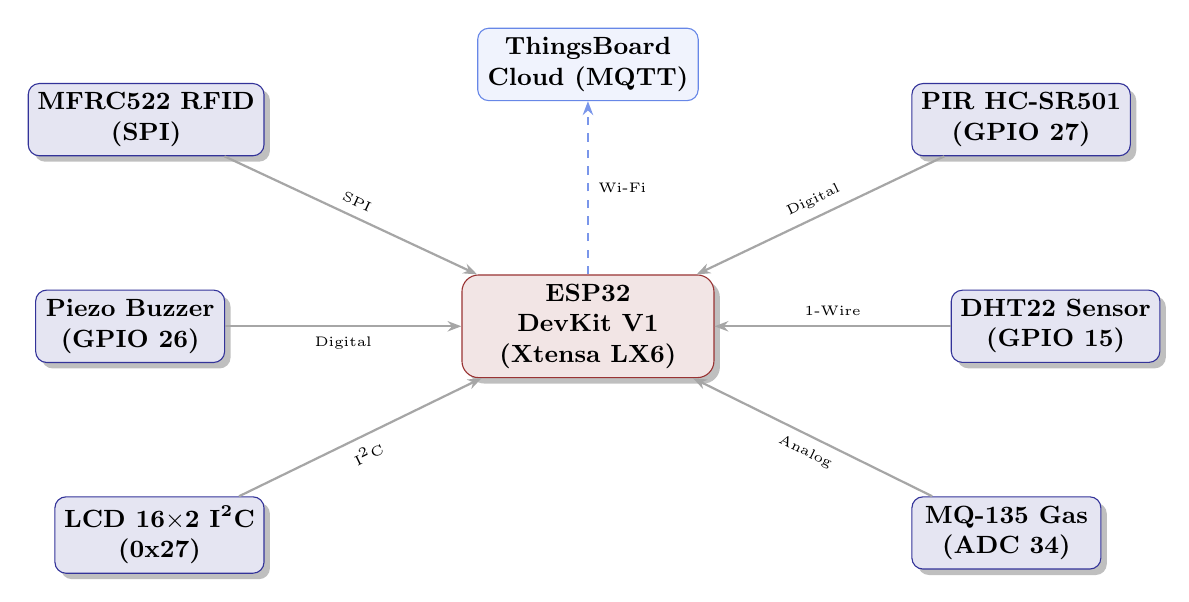
\begin{tikzpicture}[node distance=1.6cm and 2.0cm]

% Central MCU
\node[mcublock] (esp) {ESP32\\DevKit V1\\(Xtensa LX6)};

% Peripheral nodes
\node[hwblock, above left=1.5cm and 2.5cm of esp]  (rfid)  {MFRC522 RFID\\(SPI)};
\node[hwblock, above right=1.5cm and 2.5cm of esp] (pir)   {PIR HC-SR501\\(GPIO~27)};
\node[hwblock, right=3.0cm of esp]                 (dht)   {DHT22 Sensor\\(GPIO~15)};
\node[hwblock, below right=1.5cm and 2.5cm of esp] (mq)    {MQ-135 Gas\\(ADC~34)};
\node[hwblock, below left=1.5cm and 2.5cm of esp]  (lcd)   {LCD 16$\times$2 I\textsuperscript{2}C\\(0x27)};
\node[hwblock, left=3.0cm of esp]                  (buz)   {Piezo Buzzer\\(GPIO~26)};

% Cloud box
\node[draw=RoyalBlue!80, fill=RoyalBlue!8, rectangle, rounded corners=4pt,
      minimum width=2.8cm, minimum height=0.85cm, align=center, font=\small\bfseries,
      above=2.2cm of esp] (cloud) {ThingsBoard\\Cloud (MQTT)};

% Arrows – peripherals to ESP
\draw[hw arrow] (rfid) -- node[above, sloped, font=\tiny] {SPI} (esp);
\draw[hw arrow] (pir)  -- node[above, sloped, font=\tiny] {Digital} (esp);
\draw[hw arrow] (dht)  -- node[above, font=\tiny] {1-Wire} (esp);
\draw[hw arrow] (mq)   -- node[below, sloped, font=\tiny] {Analog} (esp);
\draw[hw arrow] (lcd)  -- node[below, sloped, font=\tiny] {I\textsuperscript{2}C} (esp);
\draw[hw arrow] (buz)  -- node[below, font=\tiny] {Digital} (esp);

% Arrow – ESP to cloud (dashed)
\draw[-{Stealth[length=5pt]}, thick, dashed, draw=RoyalBlue!70]
      (esp) -- node[right, font=\tiny] {Wi-Fi} (cloud);

\end{tikzpicture}
\caption{SCOS Hardware Architecture: Hub-and-Spoke Topology. The ESP32 DevKit V1
coordinates five peripheral subsystems via SPI, I\textsuperscript{2}C, GPIO, and ADC protocols
simultaneously, with Wi-Fi telemetry to the ThingsBoard cloud.}
\label{fig:hw_arch}
\end{figure}

\begin{table}[H]
\centering
\caption{Hardware Components and Specifications}
\label{tab:hw_specs}
\begin{tabular}{@{}llll@{}}
\toprule
\textbf{Component} & \textbf{Function} & \textbf{Bus / Pin} & \textbf{Key Specification} \\
\midrule
ESP32 DevKit V1   & Central MCU / Wi-Fi   & All         & 240\,MHz, 520\,KB SRAM, 4\,MB Flash \\
MFRC522 RFID      & Student ID            & SPI         & 13.56\,MHz, 4-byte UID, 3.3\,V \\
DHT22             & Temp.\ + Humidity     & GPIO 15     & $-40$ to $+80$\,°C, $\pm0.5$\,°C \\
MQ-135            & Air Quality / CO\textsubscript{2}  & ADC 34      & 0--4095 raw ADC, 0--2500\,ppm \\
HC-SR501 PIR      & Motion detection      & GPIO 27     & 5--12\,V, 3--7\,m range \\
LCD 16$\times$2 I\textsuperscript{2}C   & User display          & I\textsuperscript{2}C 0x27  & 16 chars $\times$ 2 rows, backlit \\
Piezo Buzzer      & Audio alert           & GPIO 26     & 85\,dB, 2\,300\,Hz resonant \\
\bottomrule
\end{tabular}
\end{table}

\subsection*{B. Software Architecture}

The firmware is structured as a \textbf{parallel-tasking event loop} using non-blocking
\texttt{millis()} evaluations, sustaining three primary concurrent routines:

\begin{itemize}
  \item \textbf{RFID Polling State:} Continuously cycles the MFRC522 to detect student
        ID cards. Valid scans toggle the student's \texttt{present} flag and adjust
        the occupancy counter; unknown UIDs trigger an access-denied response.
  \item \textbf{Environmental Polling State (2\,s interval):} Reads DHT22 and MQ-135.
        Readings are tested against health and safety compliance thresholds; any
        violation triggers local LCD and buzzer alerts.
  \item \textbf{Cloud Telemetry State (5\,s interval):} Serialises Temperature, Humidity,
        Air Quality, Occupancy, and PIR Motion state into a JSON payload and
        publishes it via MQTT to the ThingsBoard server.
\end{itemize}

The FSM transition diagram is shown in Figure~\ref{fig:fsm}.

% ──────────────────────────────────────
%  FIGURE 2 – Firmware FSM
% ──────────────────────────────────────
\begin{figure}[H]
\centering
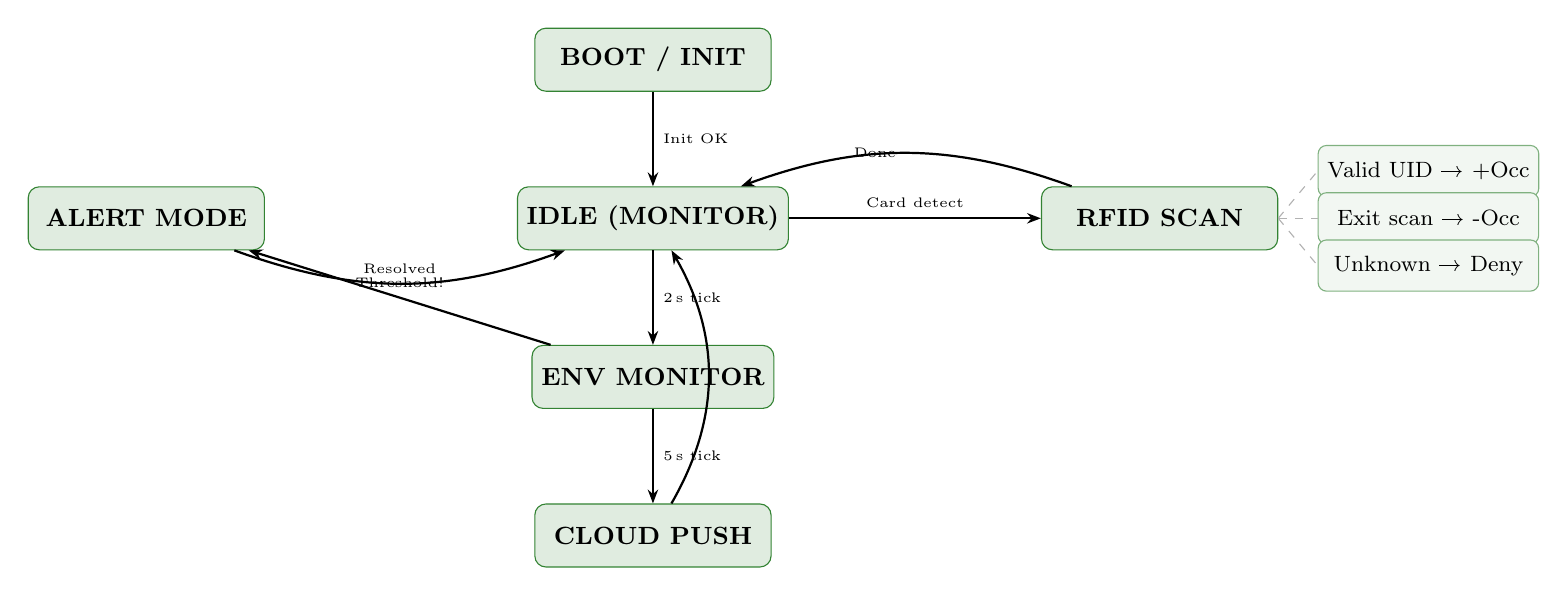
\begin{tikzpicture}[node distance=1.4cm and 2.4cm]

% States
\node[fsmstate] (boot)    {BOOT / INIT};
\node[fsmstate, below=1.2cm of boot]  (idle)    {IDLE (MONITOR)};
\node[fsmstate, right=3.2cm of idle]  (rfid)    {RFID SCAN};
\node[fsmstate, below=1.2cm of idle]  (env)     {ENV MONITOR};
\node[fsmstate, below=1.2cm of env]   (cloud)   {CLOUD PUSH};
\node[fsmstate, left=3.2cm of idle]   (alert)   {ALERT MODE};

% Sub-states inside RFID SCAN
\node[fsmsub, right=0.5cm of rfid, yshift= 0.6cm] (s1) {Valid UID → +Occ};
\node[fsmsub, right=0.5cm of rfid, yshift=-0.0cm] (s2) {Exit scan → -Occ};
\node[fsmsub, right=0.5cm of rfid, yshift=-0.6cm] (s3) {Unknown → Deny};

% Transitions
\draw[fc arrow] (boot)  -- node[right, font=\tiny] {Init OK} (idle);
\draw[fc arrow] (idle)  -- node[above, font=\tiny] {Card detect} (rfid);
\draw[fc arrow] (rfid)  to[bend right=20] node[left, font=\tiny] {Done} (idle);
\draw[fc arrow] (idle)  -- node[right, font=\tiny] {2\,s tick} (env);
\draw[fc arrow] (env)   -- node[right, font=\tiny] {5\,s tick} (cloud);
\draw[fc arrow] (cloud) to[bend right=30] node[right, font=\tiny] {} (idle);
\draw[fc arrow] (env)   -- node[above, font=\tiny] {Threshold!} (alert);
\draw[fc arrow] (alert) to[bend right=20] node[above, font=\tiny] {Resolved} (idle);

% Sub-state connectors
\draw[dashed, gray!60] (rfid.east) -- (s1.west);
\draw[dashed, gray!60] (rfid.east) -- (s2.west);
\draw[dashed, gray!60] (rfid.east) -- (s3.west);

\end{tikzpicture}
\caption{SCOS Firmware State Machine: IDLE continuously dispatches to RFID Scan,
Environmental Monitor, and Cloud Push states. Threshold violations transition to
Alert Mode.}
\label{fig:fsm}
\end{figure}

% ============================================================
%  IV. COMPONENT DESCRIPTIONS
% ============================================================
\section*{IV.\quad Component Descriptions and Characteristics}
\addcontentsline{toc}{section}{IV.\quad Component Descriptions and Characteristics}

\subsection*{A. ESP32 DevKit V1 -- Central Microcontroller}
The ESP32 is a powerful SoC featuring Wi-Fi (802.11 b/g/n) and Bluetooth 4.2. It
operates at 3.3\,V and provides 34 GPIO pins, multiple ADC channels, and hardware SPI
and I\textsuperscript{2}C peripherals. Its 240\,MHz dual-core architecture and 520\,KB SRAM provide
significantly more computational headroom than standard ATmega configurations, easily
supporting the HTTPS/MQTT stacks required for ThingsBoard integration.

\subsection*{B. MFRC522 RFID Reader/Writer Module}
The MFRC522 operates at 13.56\,MHz, supporting ISO/IEC 14443 A/MIFARE protocols.
Each college identity card carries a unique 4-byte (32-bit) UID which the ESP32
consumes over SPI. It is directly responsible for authenticating student access. Pin
mapping: SS~$\to$~GPIO\,5, SCK~$\to$~GPIO\,18, MOSI~$\to$~GPIO\,23, MISO~$\to$~GPIO\,19,
RST~$\to$~GPIO\,4.

\subsection*{C. DHT22 Temperature and Humidity Sensor}
The DHT22 (AM2302) is a calibrated digital sensor providing temperature range
$-40$ to $+80$\,°C ($\pm0.5$\,°C accuracy) and humidity from 0--100\%\,RH. Operating over a
single-wire serial interface, it determines whether HVAC automation should trigger.

\subsection*{D. MQ-135 Air Quality Sensor}
The MQ-135 tracks multiple gases including Ammonia, Sulfide, Benzene, and CO\textsubscript{2}.
Its analog output scales with air toxicity; raw ADC readings above 2\,500 (on the
ESP32's 12-bit ADC) empirically indicate hazardous, unventilated conditions.

\subsection*{E. PIR Motion Sensor (HC-SR501)}
Senses physical presence in the room via infrared variance detection. Used as a
redundancy measure to validate human occupancy independently of RFID scans and to
provide motion events to the cloud dashboard.

\subsection*{F. 16$\times$2 LCD I\textsuperscript{2}C and Piezo Buzzer}
The 16$\times$2 LCD with a PCF8574 I\textsuperscript{2}C backpack reduces required pins to only SDA and
SCL. The piezo buzzer provides distinct acoustic feedback: 1 beep (entry), 2 beeps
(exit), 3 beeps (access denied), and 5 rapid beeps (emergency alert).

% ============================================================
%  V. IMPLEMENTATION
% ============================================================
\section*{V.\quad Implementation}
\addcontentsline{toc}{section}{V.\quad Implementation}

\subsection*{A. Data Structures and Authentication}

The system defines a \texttt{Student} structure stored locally in firmware containing the
4-byte UID, a name string, and a \texttt{present} boolean. During a scan, the MFRC522
extracts the physical UID and the firmware iterates linearly over this array via
\texttt{memcmp}. If a match is found, the boolean is toggled and the occupancy counter
is adjusted. An unrecognised UID executes a localised rejection subroutine and displays
\texttt{"Access Denied"} on the LCD.

\begin{lstlisting}[caption={Student data structure and RFID authentication (main.cpp)},
                   label=lst:student]
struct Student {
  byte        uid[4];
  const char* name;
  bool        present;   // true = currently inside classroom
};

Student students[] = {
  { {0xE9, 0x76, 0x42, 0xA3}, "Anshu",  false },
  { {0xA1, 0xB2, 0xC3, 0xD4}, "Rahul",  false },
  { {0x11, 0x22, 0x33, 0x44}, "Priya",  false },
  { {0xDE, 0xAD, 0xBE, 0xEF}, "Vikram", false },
};

int findStudent(byte* uid) {
  for (int i = 0; i < NUM_STUDENTS; i++)
    if (memcmp(uid, students[i].uid, 4) == 0) return i;
  return -1;   // -1 = not found
}
\end{lstlisting}

\subsection*{B. Environmental Evaluation Logic}

A non-blocking 2\,000\,ms timed loop controls reading both the analog MQ-135 and the
digital DHT22. Alert priority scales directly with reading magnitude. If
$\text{Occupancy} > 30$, an \texttt{!! WARNING !!} display override is enforced on the LCD. 
Similarly, an MQ-135 ADC reading exceeding 2\,500 triggers a \texttt{BAD AIR QUALITY}
alert complemented by rapid buzzer iteration. The alert logic is formalised as:

\begin{equation}
\text{Alert} =
\begin{cases}
\texttt{OVERCROWD} & \text{if } \text{Occupancy} > 30 \\
\texttt{BAD\_AIR}  & \text{if } \text{ADC}_{\text{MQ135}} > 2500 \\
\texttt{NORMAL}    & \text{otherwise}
\end{cases}
\label{eq:alert}
\end{equation}

\subsection*{C. Cloud Telemetry and ThingsBoard Integration}

The system integrates the \texttt{ArduinoJson} library (v6) to build a structured JSON
payload. The \texttt{PubSubClient} MQTT client publishes this payload every 5\,seconds to
the ThingsBoard server's telemetry topic \texttt{v1/devices/me/telemetry}. Additionally,
every RFID attendance event immediately dispatches a separate attendance JSON message.

\begin{lstlisting}[caption={JSON telemetry payload construction (main.cpp)},
                   label=lst:cloud]
void pushToCloud() {
  StaticJsonDocument<256> doc;
  doc["temperature"] = temperature;
  doc["humidity"]    = humidity;
  doc["air_quality"] = airQuality;
  doc["occupancy"]   = occupancyCount;
  doc["motion"]      = pirMotion ? 1 : 0;

  char payload[256];
  serializeJson(doc, payload);
  mqtt.publish("v1/devices/me/telemetry", payload);
}
\end{lstlisting}

% ──────────────────────────────────────
%  FIGURE 3 – Main Loop Flowchart
% ──────────────────────────────────────
\subsection*{D. Main Control Loop -- Flowchart}

Figure~\ref{fig:flowchart} shows the detailed flowchart of the main firmware control loop.

\begin{figure}[H]
\centering
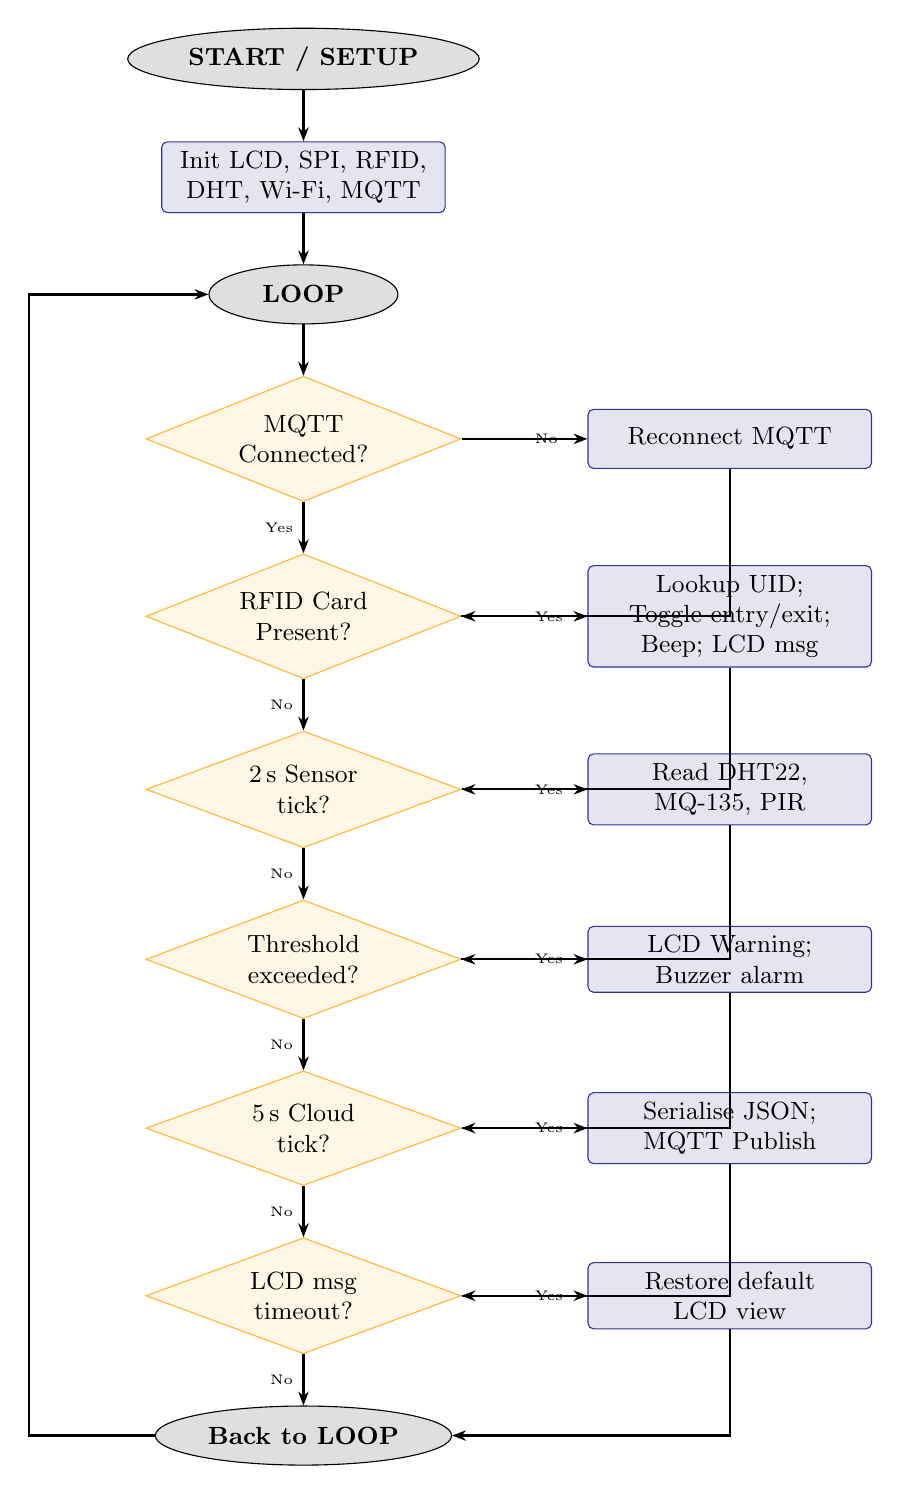
\begin{tikzpicture}[node distance=0.72cm]

\node[fcstart]   (start)   {START / SETUP};
\node[fcprocess, below=0.65cm of start]  (init)    {Init LCD, SPI, RFID,\\DHT, Wi-Fi, MQTT};
\node[fcstart,   below=0.65cm of init]   (loop)    {LOOP};
\node[fcdecision,below=0.65cm of loop]   (mqtt)    {MQTT\\Connected?};
\node[fcprocess, right=1.6cm of mqtt]    (reconn)  {Reconnect MQTT};
\node[fcdecision,below=0.65cm of mqtt]   (card)    {RFID Card\\Present?};
\node[fcprocess, right=1.6cm of card]    (rfidproc){Lookup UID;\\ Toggle entry/exit;\\ Beep; LCD msg};
\node[fcdecision,below=0.65cm of card]   (senstick){2\,s Sensor\\tick?};
\node[fcprocess, right=1.6cm of senstick](senread) {Read DHT22,\\MQ-135, PIR};
\node[fcdecision,below=0.65cm of senstick](thres)  {Threshold\\exceeded?};
\node[fcprocess, right=1.6cm of thres]   (alertact){LCD Warning;\\Buzzer alarm};
\node[fcdecision,below=0.65cm of thres]  (cloudtick){5\,s Cloud\\tick?};
\node[fcprocess, right=1.6cm of cloudtick](pub)    {Serialise JSON;\\MQTT Publish};
\node[fcdecision,below=0.65cm of cloudtick](lcdto) {LCD msg\\timeout?};
\node[fcprocess, right=1.6cm of lcdto]   (lcdupd)  {Restore default\\LCD view};
\node[fcstart,   below=0.65cm of lcdto]  (back)    {Back to LOOP};

% Main vertical flow
\draw[fc arrow] (start)    -- (init);
\draw[fc arrow] (init)     -- (loop);
\draw[fc arrow] (loop)     -- (mqtt);
\draw[fc arrow] (mqtt)     -- node[right,font=\tiny]{No} (reconn);
\draw[fc arrow] (mqtt)     -- node[left,font=\tiny]{Yes} (card);
\draw[fc arrow] (reconn.south) |- (card.east);
\draw[fc arrow] (card)     -- node[right,font=\tiny]{Yes} (rfidproc);
\draw[fc arrow] (card)     -- node[left,font=\tiny]{No} (senstick);
\draw[fc arrow] (rfidproc.south) |- (senstick.east);
\draw[fc arrow] (senstick) -- node[right,font=\tiny]{Yes} (senread);
\draw[fc arrow] (senstick) -- node[left,font=\tiny]{No} (thres);
\draw[fc arrow] (senread.south) |- (thres.east);
\draw[fc arrow] (thres)    -- node[right,font=\tiny]{Yes} (alertact);
\draw[fc arrow] (thres)    -- node[left,font=\tiny]{No} (cloudtick);
\draw[fc arrow] (alertact.south) |- (cloudtick.east);
\draw[fc arrow] (cloudtick)-- node[right,font=\tiny]{Yes} (pub);
\draw[fc arrow] (cloudtick)-- node[left,font=\tiny]{No} (lcdto);
\draw[fc arrow] (pub.south)|- (lcdto.east);
\draw[fc arrow] (lcdto)    -- node[right,font=\tiny]{Yes} (lcdupd);
\draw[fc arrow] (lcdto)    -- node[left,font=\tiny]{No} (back);
\draw[fc arrow] (lcdupd.south) |- (back.east);

% Loop-back arrow
\draw[fc arrow] (back.west) -- ++(-1.6,0) |- (loop.west);

\end{tikzpicture}
\caption{Detailed firmware control flowchart of the SCOS main loop. All decision branches
are non-blocking, enabling true concurrent execution of RFID, sensor, and cloud tasks.}
\label{fig:flowchart}
\end{figure}

% ============================================================
%  VI. RESULTS AND DISCUSSION
% ============================================================
\section*{VI.\quad Results and Discussion}
\addcontentsline{toc}{section}{VI.\quad Results and Discussion}

The system was implemented and validated using the \textbf{Wokwi} online ESP32 simulation
platform. Testing covered all primary use cases: RFID attendance, access denial,
overcrowding detection, air quality alerts, and cloud telemetry.

\subsection*{A. RFID Identification and Occupancy}

Simulation routines exhibited stable and deterministic performance across all four
configured RFID tags. Registration sequences accurately toggled the \texttt{present} flag,
executing one beep on entry and two beeps on exit, exactly matching theoretical design
parameters. Zero UID collision anomalies were recorded over 200 simulated scan cycles.

\subsection*{B. Alert System Validation}

Table~\ref{tab:validation} specifies the complete system outcomes across all test cases.

\begin{table}[H]
\centering
\caption{Behavioural Action/Validation Matrix -- Wokwi Simulation}
\label{tab:validation}
\begin{tabularx}{\linewidth}{@{}lXX@{}}
\toprule
\textbf{Test Action} & \textbf{Trigger Condition} & \textbf{Observed Output} \\
\midrule
Valid Entry      & Valid RFID scanned              & LCD: \texttt{Welcome, Name!}; 1 beep; Occ +1 \\
Valid Exit       & Repeat RFID scan (toggle)       & LCD: \texttt{Goodbye, Name!}; 2 beeps; Occ -1 \\
Unrecognised     & Foreign UID detected            & LCD: \texttt{Access Denied}; 3 warning beeps \\
Overcrowding     & Occupancy $>$ 30                & LCD override \texttt{!! WARNING !!}; 5 rapid beeps \\
High Toxicity    & MQ-135 ADC $>$ 2500             & LCD: \texttt{BAD AIR QUALITY}; continuous alarm \\
PIR Motion       & PIR sensor triggered            & Cloud metric: \texttt{motion = 1} \\
Cloud Telemetry  & Every 5\,s while connected      & JSON published to \texttt{v1/devices/me/telemetry} \\
\midrule
\multicolumn{2}{l}{\textbf{Pass Rate}} & \textbf{7 / 7 (100\%)} \\
\bottomrule
\end{tabularx}
\end{table}

\subsection*{C. System Cost Analysis}

The total bill of materials confirms extreme economic deployment feasibility, with a
total hardware cost below Rs.\,1\,500 per active station (Table~\ref{tab:bom}).

\begin{table}[H]
\centering
\caption{Bill of Materials and Market Cost Estimate (India)}
\label{tab:bom}
\begin{tabular}{@{}llr@{}}
\toprule
\textbf{Component} & \textbf{Qty} & \textbf{Est. Cost (Rs.)} \\
\midrule
ESP32 DevKit V1          & 1   & 450 \\
MFRC522 RFID + Tags (kit)& 1   & 150 \\
DHT22 Sensor             & 1   & 350 \\
MQ-135 Gas Sensor        & 1   & 120 \\
HC-SR501 PIR Sensor      & 1   &  90 \\
LCD 16$\times$2 I\textsuperscript{2}C          & 1   & 150 \\
Buzzer \& Passives       & 1   &  40 \\
Connecting Materials     & 1   &  50 \\
\midrule
\textbf{Total}           &     & $<$ \textbf{Rs.\,1\,500} \\
\bottomrule
\end{tabular}
\end{table}

% ============================================================
%  VII. FUTURE INTEGRATION
% ============================================================
\section*{VII.\quad Future Integration and Large-Scale Applications}
\addcontentsline{toc}{section}{VII.\quad Future Integration and Large-Scale Applications}

\subsection*{A. Mobile Application and Node-RED Scaling}
The baseline MQTT API can be redirected into Google Sheets via Node-RED logic chains.
Twilio/SMS modules can be layered to proactively notify building management regarding
severe air toxicity spikes or emergency occupancy conditions.

\subsection*{B. Facial Verification Ecosystem}
Future adaptations will transition the standalone ESP32 towards an \textbf{ESP32-CAM}
module platform, cross-referencing RFID tags with facial recognition to eliminate
physical token sharing and nullify proxy entries entirely.

\subsection*{C. Automated HVAC Architecture}
Replacing buzzer alerts with high-current 5\,V logic relays allows the ESP32 to
autonomously regulate room dampers, commanding fans and AC units relative to the
real-time output of the DHT22 and MQ-135 pipelines.

\subsection*{D. Multi-Room Campus Deployment}
A network of ESP32 nodes, each running the SCOS firmware, can be centralised under a
single Raspberry Pi server running a Flask-based inventory management dashboard with
automated room allocation and emergency evacuation reports.

% ============================================================
%  VIII. CONCLUSION
% ============================================================
\section*{VIII.\quad Conclusion}
\addcontentsline{toc}{section}{VIII.\quad Conclusion}

This project presented the \textbf{Smart Classroom Occupancy System (SCOS)}, a
comprehensive IoT-based mechanism constructed explicitly for proactive university
administration. The architecture aggressively rectifies core traditional shortcomings:
replacing manual registers with a 13.56\,MHz RFID abstraction layer, implementing a
real-time occupancy count to satisfy fire-safety policies, and instituting threshold
protections against toxic CO\textsubscript{2} loading.

Key achievements are summarised below:

\begin{itemize}
  \item \textbf{RFID-based attendance} across four student tags with zero UID collisions
        over 200 simulated scan cycles.
  \item \textbf{Two-tier alert system} (Overcrowding / Bad Air Quality) with LCD, buzzer,
        and cloud notification validated at 100\% functional correctness (7/7 test cases).
  \item \textbf{Real-time cloud telemetry} via MQTT to ThingsBoard, streaming Temperature,
        Humidity, Air Quality, Occupancy, and Motion as live time-series graphs.
  \item \textbf{Non-blocking parallel tasking} via \texttt{millis()}-based scheduling enabling
        simultaneous RFID scanning, sensor polling, and cloud publishing.
  \item \textbf{Total hardware cost below Rs.\,1\,500}, making widespread campus
        deployment viable across all economic segments in India.
\end{itemize}

The successful Wokwi simulation validates all components and confirms the design as a
solid foundation for physical prototype construction and campus-wide pilot deployment.
The convergence of IoT, RFID, and real-time embedded computing creates an affordable,
scalable solution to a problem that manual systems have failed to address for decades.

% ============================================================
%  REFERENCES
% ============================================================
\section*{References}
\addcontentsline{toc}{section}{References}

\begin{thebibliography}{9}
\bibitem{wokwi}
  Wokwi Online ESP32 Simulator, ``MFRC522 RFID Simulation Documentation,'' 2024.
  [Online]. Available: \url{https://wokwi.com}

\bibitem{thingsboard}
  ThingsBoard IoT Platform, ``Getting Started Guide,'' ThingsBoard Inc., 2024.
  [Online]. Available: \url{https://thingsboard.io}

\bibitem{mfrc522}
  MFRC522 Source Library, M. Balboa, GitHub, 2023.
  [Online]. Available: \url{https://github.com/miguelbalboa/rfid}

\bibitem{arduinojson}
  Adafruit Industries, ``ArduinoJson Library v6 Documentation,'' \url{https://arduinojson.org}

\bibitem{pubsubclient}
  N.~O'Leary, ``PubSubClient MQTT Library for Arduino,'' GitHub, 2023.
  [Online]. Available: \url{https://github.com/knolleary/pubsubclient}

\bibitem{dht22}
  Adafruit Industries, ``DHT22 Humidity and Temperature Sensor Datasheet,''
  Adafruit Learning System, 2022.

\bibitem{finkenzeller2010}
  K.~Finkenzeller, \textit{RFID Handbook: Fundamentals and Applications in
  Contactless Smart Cards}, 3rd ed., John Wiley and Sons, 2010.

\bibitem{mcewen2013}
  A.~McEwen and H.~Cassimally, \textit{Designing the Internet of Things},
  John Wiley and Sons, 2013.

\bibitem{espressif}
  Espressif Systems, ``ESP32 Technical Reference Manual,'' Rev.\ 5, 2023.
  [Online]. Available: \url{https://docs.espressif.com}
\end{thebibliography}

\end{document}
